%%%  کلاس AUTthesis، نسخه آبان 1397
%%%   دانشگاه صنعتی امیرکبیر                 http://www.aut.ac.ir
%%%  تالار گفتگوی پارسی‌لاتک،       http://forum.parsilatex.com
%%%   آپدیت شده در آبان 95
%%%   پشتیبانی و راهنمایی          badali_farhad@yahoo.com
%%%
%%%   بازبینی و اصلاح شده در آبان ماه 1397
%%%  Tested via TeXstudio in TeXlive 2014-2018.
%%%

%-----------------------------------------------------------------------------------------------------
%        روش اجرا.: 2 بار F1 ، 2 بار  F11(به منظور تولید مراجع) ، دوبار Ctrl+Alt+I (به منظور تولید نمایه) و دو بار F1 -------> مشاهده Pdf
%%%%%%%%%%%%%%%%%%%%%%%%%%%%%%%%%%%%%%%%%%%%%%%%%%%%%%
%   TeXstudio as your IDE
%%  برای compile در TeXstudio تنها کافی است منوی Options->Configure TeXstudio را زده و در پنجره Configure TeXstudio در بخش Build گزینه Default Compiler را به XeLaTeX تغییر دهید. سند شما به راحتی compile خواهد شد.
%   F1 & F5 : Build & view
%   F6      : Compile
%   F7      : View
%   --------------
%%%%%%%%%%%%%%%%%%%%%%%%%%%%%%%%%%%%%%%%%%%%%%%%%%%%%%
%        اگر قصد نوشتن رساله دکتری را دارید، در خط زیر به جای msc،
%      کلمه phd را قرار دهید. کلیه تنظیمات لازم، به طور خودکار، اعمال می‌شود.
%%% !TEX TS-program = XeLaTeX
\documentclass[oneside,bsc,12pt]{AUTthesis}
%       فایل commands.tex را حتماً به دقت مطالعه کنید؛ چون دستورات مربوط به فراخوانی بسته زی‌پرشین 
%       و دیگر بسته‌ها و ... در این فایل قرار دارد و بهتر است که با نحوه استفاده از آنها آشنا شوید. توجه شود برای نسخه نهایی پایان‌نامه حتماً hyperref را 
%        غیرفعال کنید.


% در این فایل، دستورها و تنظیمات مورد نیاز، آورده شده است.
%-------------------------------------------------------------------------------------------------------------------
% در ورژن جدید زی‌پرشین برای تایپ متن‌های ریاضی، این سه بسته، حتماً باید فراخوانی شود.
\usepackage{amsthm,amssymb,amsmath,amsfonts}
% بسته‌ای برای تنطیم حاشیه‌های بالا، پایین، چپ و راست صفحه
\usepackage[top=30mm, bottom=30mm, left=25mm, right=30mm]{geometry}
% بسته‌‌ای برای ظاهر شدن شکل‌ها و تصاویر متن
\usepackage{graphicx}
\usepackage{color}
%بسته‌ای برای تنظیم فاصله عمودی خط‌های متن
\usepackage{setspace}
\usepackage{titletoc}
\usepackage{tocloft}
%با فعال کردن بسته زیر فوت‌نوت‌ها در هر صفحه ریست می‌شوند. حالت پیش‌فرض آن ریست شدن در هر فصل می‌باشد.
%\usepackage[perpage]{footmisc}
\usepackage{enumitem}
%\usepackage{titlesec}
% بسته‌ و دستوراتی برای ایجاد لینک‌های رنگی با امکان جهش
\usepackage[pagebackref=false,colorlinks,linkcolor=blue,citecolor=red]{hyperref}
\usepackage[nameinlink]{cleveref}%capitalize,,noabbrev
 \AtBeginDocument{%
    \crefname{equation}{برابری}{equations}%
    \crefname{chapter}{فصل}{chapters}%
    \crefname{section}{بخش}{sections}%
    \crefname{appendix}{پیوست}{appendices}%
    \crefname{enumi}{مورد}{items}%
    \crefname{footnote}{زیرنویس}{footnotes}%
    \crefname{figure}{شکل}{figures}%
    \crefname{table}{جدول}{tables}%
    \crefname{theorem}{قضیه}{theorems}%
    \crefname{lemma}{لم}{lemmas}%
    \crefname{corollary}{نتیجه}{corollaries}%
    \crefname{proposition}{گزاره}{propositions}%
    \crefname{definition}{تعریف}{definitions}%
    \crefname{result}{نتیجه}{results}%
    \crefname{example}{مثال}{examples}%
    \crefname{remark}{نکته}{remarks}%
    \crefname{note}{یادداشت}{notes}%
}
% چنانچه قصد پرینت گرفتن نوشته خود را دارید، خط بالا را غیرفعال و  از دستور زیر استفاده کنید چون در صورت استفاده از دستور زیر‌‌، 
% لینک‌ها به رنگ سیاه ظاهر خواهند شد که برای پرینت گرفتن، مناسب‌تر است
%\usepackage[pagebackref=false]{hyperref}
% بسته‌ لازم برای تنظیم سربرگ‌ها
\usepackage{fancyhdr}
% بسته‌ای برای ظاهر شدن «مراجع»  در فهرست مطالب
\usepackage[nottoc]{tocbibind}
% دستورات مربوط به ایجاد نمایه
\usepackage{makeidx,multicol}
\setlength{\columnsep}{1.5cm}

%%%%%%%%%%%%%%%%%%%%%%%%%%
\usepackage{verbatim}
\makeindex
\usepackage{sectsty}
% فراخوانی بسته زی‌پرشین و تعریف قلم فارسی و انگلیسی
\usepackage{xepersian}%[extrafootnotefeatures]
\SepMark{-}
%حتماً از تک لایو 2014 استفاده کنید.
\settextfont[Scale=1.2]{B Nazanin.ttf}
\setlatintextfont{Times New Roman.ttf}
\renewcommand{\labelitemi}{$\bullet$}
%%%%%%%%%%%%%%%%%%%%%%%%%%
% چنانچه می‌خواهید اعداد در فرمول‌ها، انگلیسی باشد، خط زیر را غیرفعال کنید.
%در غیر اینصورت حتماً فونت PGaramond را نصب کنید.
%\setdigitfont[Scale=1.1]{PGaramond.ttf}%%Yas
%\setdigitfont[Scale=1.1]{Yas.ttf}%%Yas
%%%%%%%%%%%%%%%%%%%%%%%%%%
% تعریف قلم‌های فارسی اضافی برای استفاده در بعضی از قسمت‌های متن
\defpersianfont\nastaliq[Scale=2]{IranNastaliq.ttf}
\defpersianfont\chapternumber[Scale=3]{B Nazanin.ttf}
%\chapterfont{\centering}%
%%%%%%%%%%%%%%%%%%%%%%%%%%
% دستوری برای تغییر نام کلمه «اثبات» به «برهان»
\renewcommand\proofname{\textbf{برهان}}

% دستوری برای تغییر نام کلمه «کتاب‌نامه» به «منابع و مراجع«
\renewcommand{\bibname}{منابع و مراجع}


% Headings for every page of ToC, LoF and Lot
\setlength{\cftbeforetoctitleskip}{-1.2em}
\setlength{\cftbeforelottitleskip}{-1.2em}
\setlength{\cftbeforeloftitleskip}{-1.2em}
\setlength{\cftaftertoctitleskip}{-1em}
\setlength{\cftafterlottitleskip}{-1em}
\setlength{\cftafterloftitleskip}{-1em}
%%\makeatletter
%%%%\renewcommand{\l@chapter}{\@dottedtocline{1}{1em\bfseries}{1em}}
%%%%\renewcommand{\l@section}{\@dottedtocline{2}{2em}{2em}}
%%%%\renewcommand{\l@subsection}{\@dottedtocline{3}{3em}{3em}}
%%%%\renewcommand{\l@subsubsection}{\@dottedtocline{4}{4em}{4em}}
%%%%\makeatother


\newcommand\tocheading{\par عنوان\hfill صفحه \par}
\newcommand\lofheading{\hspace*{.5cm}\figurename\hfill صفحه \par}
\newcommand\lotheading{\hspace*{.5cm}\tablename\hfill صفحه \par}

\renewcommand{\cftchapleader}{\cftdotfill{\cftdotsep}}
\renewcommand{\cfttoctitlefont}{\hspace*{\fill}\LARGE\bfseries}%\Large
\renewcommand{\cftaftertoctitle}{\hspace*{\fill}}
\renewcommand{\cftlottitlefont}{\hspace*{\fill}\LARGE\bfseries}%\Large
\renewcommand{\cftafterlottitle}{\hspace*{\fill}}
\renewcommand{\cftloftitlefont}{\hspace*{\fill}\LARGE\bfseries}
\renewcommand{\cftafterloftitle}{\hspace*{\fill}}

%%%%%%%%%%%%%%%%%%%%%%%%%%
% تعریف و نحوه ظاهر شدن عنوان قضیه‌ها، تعریف‌ها، مثال‌ها و ...
%برای شماره گذاری سه تایی قضیه ها
\theoremstyle{definition}
\newtheorem{definition}{تعریف}[section]
\newtheorem{remark}[definition]{نکته}
\newtheorem{note}[definition]{یادداشت}
\newtheorem{example}[definition]{نمونه}
\newtheorem{question}[definition]{سوال}
\newtheorem{remember}[definition]{یاداوری}
\theoremstyle{theorem}
\newtheorem{theorem}[definition]{قضیه}
\newtheorem{lemma}[definition]{لم}
\newtheorem{proposition}[definition]{گزاره}
\newtheorem{corollary}[definition]{نتیجه}
%%%%%%%%%%%%%%%%%%%%%%%%
%%%%%%%%%%%%%%%%%%%
%%% برای شماره گذاری چهارتایی قضیه ها و ...
%%\newtheorem{definition1}[subsubsection]{تعریف}
%%\newtheorem{theorem1}[subsubsection]{قضیه}
%%\newtheorem{lemma1}[subsubsection]{لم}
%%\newtheorem{proposition1}[subsubsection]{گزاره}
%%\newtheorem{corollary1}[subsubsection]{نتیجه}
%%\newtheorem{remark1}[subsubsection]{نکته}
%%\newtheorem{example1}[subsubsection]{مثال}
%%\newtheorem{question1}[subsubsection]{سوال}

%%%%%%%%%%%%%%%%%%%%%%%%%%%%

% دستورهایی برای سفارشی کردن صفحات اول فصل‌ها
\makeatletter
\newcommand\mycustomraggedright{%
 \if@RTL\raggedleft%
 \else\raggedright%
 \fi}
\def\@makechapterhead#1{%
\thispagestyle{style1}
\vspace*{20\p@}%
{\parindent \z@ \mycustomraggedright
\ifnum \c@secnumdepth >\m@ne
\if@mainmatter

\bfseries{\Huge \@chapapp}\small\space {\chapternumber\thechapter}
\par\nobreak
\vskip 0\p@
\fi
\fi
\interlinepenalty\@M 
\Huge \bfseries #1\par\nobreak
\vskip 120\p@

}

%\thispagestyle{empty}
\newpage}
\bidi@patchcmd{\@makechapterhead}{\thechapter}{\tartibi{chapter}}{}{}
\bidi@patchcmd{\chaptermark}{\thechapter}{\tartibi{chapter}}{}{}
\makeatother

\pagestyle{fancy}
\renewcommand{\chaptermark}[1]{\markboth{\chaptername~\tartibi{chapter}: #1}{}}

\fancypagestyle{style1}{
\fancyhf{} 
\fancyfoot[c]{\thepage}
\fancyhead[R]{\leftmark}%
\renewcommand{\headrulewidth}{1.2pt}
}


\fancypagestyle{style2}{
\fancyhf{}
\fancyhead[R]{چکیده}
\fancyfoot[C]{\thepage{}}
\renewcommand{\headrulewidth}{1.2pt}
}

\fancypagestyle{style3}{%
  \fancyhf{}%
  \fancyhead[R]{فهرست نمادها}
  \fancyfoot[C]{\thepage}%
  \renewcommand{\headrulewidth}{1.2pt}%
}

\fancypagestyle{style4}{%
  \fancyhf{}%
  \fancyhead[R]{فهرست جداول}
  \fancyfoot[C]{\thepage}%
  \renewcommand{\headrulewidth}{1.2pt}%
}

\fancypagestyle{style5}{%
  \fancyhf{}%
  \fancyhead[R]{فهرست اشکال}
  \fancyfoot[C]{\thepage}%
  \renewcommand{\headrulewidth}{1.2pt}%
}

\fancypagestyle{style6}{%
  \fancyhf{}%
  \fancyhead[R]{فهرست مطالب}
  \fancyfoot[C]{\thepage}%
  \renewcommand{\headrulewidth}{1.2pt}%
}

\fancypagestyle{style7}{%
  \fancyhf{}%
  \fancyhead[R]{نمایه}
  \fancyfoot[C]{\thepage}%
  \renewcommand{\headrulewidth}{1.2pt}%
}

\fancypagestyle{style8}{%
  \fancyhf{}%
  \fancyhead[R]{منابع و مراجع}
  \fancyfoot[C]{\thepage}%
  \renewcommand{\headrulewidth}{1.2pt}%
}
\fancypagestyle{style9}{%
  \fancyhf{}%
  \fancyhead[R]{واژه‌نامه‌ی فارسی به انگلیسی}
  \fancyfoot[C]{\thepage}%
  \renewcommand{\headrulewidth}{1.2pt}%
}
%


%دستور حذف نام لیست تصاویر و لیست جداول از فهرست مطالب
\newcommand*{\BeginNoToc}{%
  \addtocontents{toc}{%
    \edef\protect\SavedTocDepth{\protect\the\protect\value{tocdepth}}%
  }%
  \addtocontents{toc}{%
    \protect\setcounter{tocdepth}{-10}%
  }%
}
\newcommand*{\EndNoToc}{%
  \addtocontents{toc}{%
    \protect\setcounter{tocdepth}{\protect\SavedTocDepth}%
  }%
}
\newcounter{savepage}
\renewcommand{\listfigurename}{فهرست اشکال}
\renewcommand{\listtablename}{فهرست جداول}
%\renewcommand\cftsecleader{\cftdotfill{\cftdotsep}}
%%%%%%%%%%%%%%%%%%%%%%%%%%%%%
%%%%%%%%%%%%%%%%%%%%%%%%%%%%

\begin{document}
\baselineskip=.75cm
\linespread{1.75}
%% -!TEX root = AUTthesis.tex
% در این فایل، عنوان پایان‌نامه، مشخصات خود، متن تقدیمی‌، ستایش، سپاس‌گزاری و چکیده پایان‌نامه را به فارسی، وارد کنید.
% توجه داشته باشید که جدول حاوی مشخصات پروژه/پایان‌نامه/رساله و همچنین، مشخصات داخل آن، به طور خودکار، درج می‌شود.
%%%%%%%%%%%%%%%%%%%%%%%%%%%%%%%%%%%%
% دانشکده، آموزشکده و یا پژوهشکده  خود را وارد کنید
\faculty{دانشکده مهندسی کامپیوتر}
% گرایش و گروه آموزشی خود را وارد کنید
\department{}
% عنوان پایان‌نامه را وارد کنید
\fatitle{روش‌های انتخاب ویژگی برای مسائل دسته‌بندی متن}
% نام استاد(ان) راهنما را وارد کنید
\firstsupervisor{دکتر محمد رحمتی}
%\secondsupervisor{استاد راهنمای دوم}
% نام استاد(دان) مشاور را وارد کنید. چنانچه استاد مشاور ندارید، دستور پایین را غیرفعال کنید.
%\firstadvisor{نام کامل استاد مشاور}
%\secondadvisor{استاد مشاور دوم}
% نام نویسنده را وارد کنید
\name{علیرضا }
% نام خانوادگی نویسنده را وارد کنید
\surname{مازوچی}
%%%%%%%%%%%%%%%%%%%%%%%%%%%%%%%%%%
\thesisdate{بهمن 1400}

% چکیده پایان‌نامه را وارد کنید
\fa-abstract{
در اين قسمت چكيده پایان نامه نوشته مي‌شو‌د‌.‌ چكيده بايد جامع و بيان‌كننده‌ خلاصه‌اي از اقدامات انجام‌شده باشد. در چكيده باید از ارجاع به مرجع و ذكر روابط رياضي، بيان تاريخچه و تعريف مسئله خودداري ‌شود. 
}


% کلمات کلیدی پایان‌نامه را وارد کنید
\keywords{کلیدواژه اول، ...، کلیدواژه پنجم (نوشتن سه تا پنج واژه کلیدی ضروری است)}



\AUTtitle
%%%%%%%%%%%%%%%%%%%%%%%%%%%%%%%%%%
\vspace*{7cm}
\thispagestyle{empty}
\begin{center}

\includegraphics[height=5cm,width=12cm]{besm}
\end{center}
% تاییدیه دفاع
\newpage
\thispagestyle{empty}
%\fontsize{18pt}{19pt}\selectfont

\section*{صفحه فرم ارزیابی و تصویب پایان نامه- فرم تأیید اعضاء كميته دفاع}

\fontsize{12pt}{14pt}\selectfont
%\renewcommand{\baselinestretch}{1.5}
\vspace*{1cm}
   در این صفحه فرم دفاع یا تایید و تصویب پایان نامه موسوم به فرم کمیته دفاع- موجود در پرونده آموزشی- را قرار دهید.
\vspace*{1cm}


\subsection*{نکات مهم:}
 
\begin{itemize}
\item
	نگارش پایان نامه/رساله باید به
	{\color{red}
		زبان فارسی
	}
	و بر اساس آخرین نسخه دستورالعمل و راهنمای تدوین پایان نامه های دانشگاه صنعتی امیرکبیر باشد.(دستورالعمل و راهنمای حاضر)
\item رنگ جلد پایان نامه/رساله چاپي كارشناسي، كارشناسي ارشد و دكترا  بايد به ترتيب مشكي، طوسي و سفيد رنگ باشد.  
\item چاپ و صحافی پایان نامه/رساله بصورت
{\color{red}
	پشت و رو(دورو)
}
بلامانع است و انجام آن توصيه مي شود. 
\end{itemize}
%%%%%%%%%%%%%%%%%%%%%%%%%%%%%%%%%%%%%%%%%%%%%%%%%%%%%%%%%%%%%%%%%%%%%%%%%%%%%%%%%%%%%%%%%%%%%%%%%%
%%%%%%%%%%%%%%%%%%%%%%%%%%%%%%%%%%%%%%%%%%%%%%%%%%%%%%%%%%%%%%%%%%%%%%%%%%%%%%%%%%%%%%%%%%%%%%%%%%
\newpage
\thispagestyle{empty}
\begin{picture}(50,50)
  \put(17,0){
\includegraphics[scale=1.1]{fa-logo}}
  \put(4.5,-13){\footnotesize{دانشگاه صنعتی امیرکبیر}}
  \put(10.5,-27){\footnotesize{(پلی‌تکنیک تهران)}}
  \put(170,30){\bf{به نام خدا}}
  \put(140,-5){\Large\bf{تعهدنامه اصالت اثر}}
  \put(310,0){تاریخ: \datethesis}
\end{picture}

\vspace*{2.5cm}

اينجانب {\bf{\fname\lname}} متعهد می‌شوم که مطالب مندرج در این پایان‌نامه حاصل کار پژوهشی اینجانب تحت نظارت و راهنمایی اساتید دانشگاه صنعتی امیرکبیر بوده و به دستاوردهای دیگران که در این پژوهش از آنها استفاده شده است مطابق مقررات و روال متعارف ارجاع و در فهرست منابع و مآخذ ذکر گردیده است. این پایان‌نامه قبلاً برای احراز هیچ مدرک هم‌سطح یا بالاتر ارائه نگردیده است.

در صورت اثبات تخلف در هر زمان، مدرک تحصیلی صادر شده توسط دانشگاه از درجه اعتبار ساقط بوده و دانشگاه حق پیگیری قانونی خواهد داشت.


کلیه نتایج و حقوق حاصل از این پایان‌نامه متعلق به دانشگاه صنعتی امیرکبیر می‌باشد. هرگونه استفاده از نتایج علمی و عملی، واگذاری اطلاعات به دیگران یا چاپ و تکثیر، نسخه‌برداری، ترجمه و اقتباس از این پایان نامه بدون موافقت کتبی دانشگاه صنعتی امیرکبیر ممنوع است. 
نقل مطالب با ذکر مآخذ بلامانع است.\\
\vspace{2.5cm}


{\centerline {\bf{\fname\lname}}}
\vspace*{.2cm}
{\centerline{امضا}}
%%%%%%%%%%%%%%%%%%%%%%%%%%%%%%%%%
% چنانچه مایل به چاپ صفحات «تقدیم»، «نیایش» و «سپاس‌گزاری» در خروجی نیستید، خط‌های زیر را با گذاشتن ٪  در ابتدای آنها غیرفعال کنید.
% پایان‌نامه خود را تقدیم کنید
% نیایش خود را در فایل زیر بنویسید.
\begin{acknowledgementpage}

\vspace{1.5cm}

{\nastaliq
{
 نويسنده پايان‌نامه، درصورت تمايل ميتواند برای سپاسگزاری پايان‌نامه خود را به شخص يا اشخاص و يا ارگان خاصی تقدیم نماید.
}}\end{acknowledgementpage}
\newpage
% سپاسگزاری را در فایل زیر بنویسید.
%%%%%%%%%%%%%%%%%%%%%%%%%%%%%%%%%%%%
%\newpage\thispagestyle{empty}
% سپاس‌گزاری
%{\nastaliq
%سپاس‌گزاری
%}
%\\[2cm]














% با استفاده از دستور زیر، امضای شما، به طور خودکار، درج می‌شود.
%\signature








%%%%%%%%%%%%%%%%%%%%%%%%%%%%%%%%%%%%%%%%%
%%%%%%%%%%%%%%%%%%%%%%%%%%%%%%%%%کدهای زیر را تغییر ندهید.
\newpage\clearpage

\pagestyle{style2}

\vspace*{-1cm}
\section*{\centering چکیده}
%\addcontentsline{toc}{chapter}{چکیده}
\vspace*{.5cm}
\ffa-abstract
\vspace*{2cm}


{\noindent\large\textbf{واژه‌های کلیدی:}}\par
\vspace*{.5cm}
\fkeywords
% دستور زیر برای شماره گذاری صفحات قبل از فصل اول با حروف ابجد است.
\pagenumbering{alph}
%-----------------------------------------------------------------------------
% فایل زیر دستورات مربوط به نمایش صفحات فهرست مطالب- فهرست اشکال و جداول است.
%{\pagestyle{style2}
%\tableofcontents}\newpage
%
%\listoffigures
\cleardoublepage
\pagestyle{style6}
\tableofcontents
\pagestyle{style6}
\cleardoublepage
%اگر لیست تصاویر و لیست جداول ندارید ، کدهای زیر را با گذاشتن % در ابتدای آنها، غیرفعال کنید.
\BeginNoToc
%============
%\addtocontents{lof}{\lofheading}% add heading to the first page in LoF
%\pagestyle{style5}
%\listoffigures
%\thispagestyle{style5}
%\cleardoublepage
%============
\addtocontents{lot}{\lotheading}% add heading to the first page in LoT
\thispagestyle{style4}
\listoftables
\thispagestyle{style4}
%============
%\cleardoublepage
%
\cleardoublepage
\setcounter{savepage}{\arabic{page}}
\mainmatter
\addtocontents{toc}{\tocheading}% add heading to the first page in ToC, after frontmatter entries
\EndNoToc
% در صورت تمایل می‌توانید با فعال کردن دستور بالا، لیست تصاویر را به  پایان‌نامه خود اضافه کنید.
%-------------------------------------------------------------------------symbols(فهرست نمادها)
% وجود لیست نمادها الزامیست.(لطفاً نمادهای خود را جایگذین نمادهای پیش‌فرض کنید.)
%%%%%%%%%%%%%

{\centering\LARGE\textbf{فهرست نمادها}\par}%

\pagenumbering{alph}
\setcounter{page}{\thesavepage}
%\setcounter{page}{6}
\vspace*{1cm}

\pagestyle{style3}
%\thispagestyle{empty}
%\addcontentsline{toc}{chapter}{فهرست نمادها}
\symb{\text{ نماد}}{مفهوم}
\\
%مقادیر بالا را تغییر ندهید
%%%%%%%%%%%%%%%%%%%%%%%%%%%%%%%%%%%%%%%%%%%%%%%%%%%%%%%%%
\symb{\mathbb{R}^n}{
فضای اقلیدسی با بعد $n$
}
\symb{\mathbb{S}^n}{
کره یکه $n$ بعدی
}
\symb{M^m}{
خمینه $m$-بعدی $M$
}
\symb{\mathfrak{X}(M)}{
جبر میدان‌های  برداری هموار روی $M$
}
\symb{\mathfrak{X}^1(M)}{
مجموعه میدان‌های برداری هموار یکه روی $(M,g)$ 
}
\symb{\Omega^p(M)}{
مجموعه $p$-فرمی‌های روی خمینه $M$
}
\symb{Q}{
اپراتور ریچی
}
\symb{\mathcal{R}}{
تانسور انحنای ریمان
}
\symb{ric}{
تانسور ریچی
}
\symb{L}{
مشتق لی
}
\symb{\Phi}{
2-فرم اساسی خمینه تماسی
}
\symb{\nabla}{
التصاق لوی-چویتای
}
\symb{\Delta}{
لاپلاسین ناهموار
}
\symb{\nabla^*}{
عملگر خودالحاق صوری القا شده از التصاق لوی-چویتای
}
\symb{g_s}{
متر ساساکی
}
\symb{\nabla}{
التصاق لوی-چویتای وابسته به متر ساساکی
}
\symb{\Delta}{
عملگر لاپلاس-بلترامی روی $p$-فرم‌ها
}

%%%%%%%%%%%%%%%%%%%%%%%%%%%%%%%%%%%%%%%

\thispagestyle{style3}
\newpage
%\pagestyle{style1}
%%%%%%%%%%%%%%%%%%%%%%%%%%%%%%%%%%%%


\pagenumbering{arabic}
\pagestyle{style1}
%--------------------------------------------------------------------------chapters(فصل ها)
\chapter{مقدمه}

\chapter{مفاهیم تئوری}
در این بخش قصد داریم در مورد مفاهیم تئوری که در روش‌های مورد بررسی این پروژه استفاده شده‌اند بپردازیم. به طور دقیق‌تر ابتدا در مورد روش‌های انتخاب ویژگی معروف صحبت خواهد شد و سپس الگوریتم ژنتیک توضیح داده می‌شود.


\section{دسته‌بندی روش‌های انتخاب ویژگی}
روش‌های انتخاب ویژگی به چندین دسته تقسیم می‌شوند. دو روش متداول و شناخته‌شده‌تر آن روش‌های فیلتر\LTRfootnote{Filter} و پوشاننده\LTRfootnote{Wrapper} هستند. در روش‌های پوشاننده مستقیما ویژگی‌های انتخاب‌شده را در یک مسئله واقعی (که در اینجا یک مسئله دسته‌بندی متن است) استفاده می‌کنند و لذا امتیازی که برای یک مجموعه ویژگی انتخاب‌شده بدست می‌آید امتیاز دقت واقعی برای مسئله دسته‌بندی است. در مقابل و در روش‌های فیلتر،‌ با اعمال روش‌های آماری سعی می‌شود که یک امتیاز برای یک مجموعه ویژگی انتخاب‌شده حاصل گردد.
\\

روش‌های پوشاننده چون به صورت مستقیم مجموعه ویژگی را بررسی می‌کند منجر به خروجی دقیق‌تری می‌شود؛ اما باید توجه داشت که روش‌های فیلتر زمان اجرای به مراتب بهتری دارند و بر روی مسئله دسته‌بندی بایاس نخواهند شد\cite{labani2018novel}. در مسائل دسته‌بندی چون تعداد ویژگی‌ها بسیار بالاست نمی‌توان از روش‌های پوشاننده مستقیم استفاده کرد و لذا یا باید از روش‌های فیلتر استفاده کرد و یا به صورت ترکیبی از این دو شیوه بهره گرفت.
\\

روش‌های فیلتر خود به چندین دسته قابل تقسیم هستند؛ نخست آنکه می‌توان این روش‌ها را به روش‌های محلی\LTRfootnote{Local} و روش‌های جهانی\LTRfootnote{Global} تقسیم کرد. در روش‌های جهانی به ویژگی یک امتیاز مطلق داده می‌شود، اما در روش‌های محلی به هر ویژگی متناسب با هر کلاس یک امتیاز داده می‌شود؛ یعنی در روش‌های محلی مشخص است که یک ویژگی برای هر کلاس تا چه میزان خاصیت متمایزکننده دارد. در حالتی که از یک معیار محلی استفاده می‌شود می‌توان مشخص کرد که یک ویژگی می‌توان عضویت یک متن به یک کلاس را نشان دهد یا آنکه عدم عضویت را می‌تواند به خوبی نشان دهد. اگر عضویت را بتواند بهتر نشان دهد آن را یک ویژگی مثبت\LTRfootnote{Positive} و در غیر این صورت آن را یک ویژگی منفی\LTRfootnote{Negative} برای آن کلاس به حساب می‌آورند.\cite{uysal2016improved}.
\\

روش‌های فیلتر را می‌توان به دو دسته تک متغیره\LTRfootnote{Univariate} و چندمتغیره \LTRfootnote{Multivariate} هم تقسیم کرد. در روش‌های تک متغیره هر ویژگی به صورت مستقل از سایر ویژگی‌ها امتیاز دریافت می‌کند، ولی در روش‌های چند متغیره در کنار آن که به شباهت ویژگی به هدف نگاه می‌شود، به زائد نبودن ویژگی‌ها نسبت به یکدیگر هم توجه می‌شود.\cite{labani2018novel}

\section{محاسبه روش‌های انتخاب ویژگی}
در این بخش مهم‌ترین معیار‌های انتخاب ویژگی معرفی می‌شوند و نحوه محاسبه آن‌ها ارائه می‌شود. این معیار‌ها تماما جز روش‌های انتخاب ویژگی فیلتر هستند.

\subsection{بهره اطلاعاتی}
بهره اطلاعاتی\LTRfootnote{Information Gain}
یکی از معیارهای محبوب برای انتخاب ویژگی در مقالات است
\cite{labani2018novel}\cite{uysal2016improved}\cite{ghareb2016hybrid}.
نحوه محاسبه این معیار برای یک کلمه در رابطه ۲-۱ آمده است.

\begin{equation}
IG(t) = -\sum_{i=1}^M P(C_i)\log{P(C_i)} + P(t)\sum_{i=1}^M P(C_i|t)\log{P(C_i|t)} + P(\bar{t})\sum_{i=1}^M P(C_i|\bar{t})\log{P(C_i|\bar{t})}
\end{equation}

در این رابطه
$IG(t)$
به معنای مقدار بهره اطلاعاتی برای کلمه
$t$
است. 
$M$
  برابر با تعداد کلاس‌ها است.
$P(C_i)$
احتمال کلاس
$C_i$
است؛ یعنی چه تعدادی از اسناد به این کلاس تعلق دارند.
$P(t)$
احتمال مربوط به کلمه
$t$
است؛ یعنی آنکه چه تعدادی از اسناد شامل این کلمه هستند. به طور مشابه 
$P(\bar{t})$
به معنای احتمال عدم این کلمه است؛ یعنی آنکه چه تعدادی از اسناد شامل این کلمه نیستند.
$P(C_i|t)$
احتمال کلاس
$C_i$
به شرط کلمه
$t$
است؛ بدین معنا که چه تعدادی از اسناد شامل کلمه
$t$
به کلاس
$C_i$
تعلق دارند.
به طور مشابه
$P(C_i|\bar{t})$
هم تعریف می‌شود.

\subsection{شاخص جینی}
 شاخص جینی\LTRfootnote{Gini index}
معیاری دیگر برای انتخاب ویژگی است که در مقالاتی مورد استفاده قرار گرفته است
\cite{labani2018novel}\cite{uysal2016improved}.
نحوه محاسبه این معیار در رابطه ۲-۲ آورده شده است.

\begin{equation}
GI(t) = \sum_{i=1}^M P(t|C_i)^2 P(C_i|t)^2
\end{equation}

در این رابطه 
$GI(t)$
به معنای مقدار شاخص جینی برای کلمه
$t$
است. 
$P(t|C_i)$
احتمال شرطی کلمه 
$t$
نسبت به کلاس
$C_i$
است؛ بدین تعریف که بررسی می‌کند که چه تعداد از اسناد متعلق به کلاس 
$C_i$
دارای کلمه
$t$
هستند. سایر نماد‌های این رابطه در بخش قبل تعریف شده است.

\subsection{نسبت نابرابری}
نسبت نابرابری
\LTRfootnote{Odds Ration}
معیاری است که برای انتخاب ویژگی در مقاله اویسال
\LTRfootnote{Uysal}
  و مقاله غارب و همکاران \LTRfootnote{Ghareb} استفاده شده است
\cite{uysal2016improved}\cite{ghareb2016hybrid}
. نحوه محاسبه این معیار در رابطه ۲-۳ آورده شده است.

\begin{equation}
OR(t, C_i) = \log{\frac{P(t|C_i)[1-P(t|\bar{C_i})]}{[1-P(t|C_i)]P(t|\bar{C_i})}}
\end{equation}

در این رابطه
$OR(t, C_i)$
نسبت نابرابری به ازای کلمه
$t$
و کلاس
$C_i$
محاسبه شده است. در کار تحقیقاتی اویسال برای جلوگیری از صفر شدن مخرج مقدار 0/01 به صورت و مخرج افزوده شده است
\cite{uysal2016improved}
.

\subsection{معیار زائدی کمینه شباهت بیشینه}
معیار زائدی کمینه شباهت بیشینه
\LTRfootnote{Minimal redundancy maximal relevance}
که با نماد 
$mRMR$
یک روش انتخاب ویژگی چند متغیره است که در مقاله لبنی و همکاران مورد استفاده قرار گرفته است
\cite{labani2018novel}
. نحوه محاسبه این معیار در رابطه ۲-۴ آمده است.
\begin{equation}
mRMR(f_j) = I(f_j, C_k) - \frac{1}{|S|-1} \sum_{f_i \in S} I(f_i, f_j)
\end{equation}

در این رابطه مجموعه
$S$
به معنی مجموعه ویژگی‌های انتخابی است.
$I(a, b)$
به معنای اطلاعات متقابل
\LTRfootnote{Mutual information}
$a$
و
$b$
است.

اگر به منطق این رابطه نگاه کنیم، در می‌یابیم با این معیار به دنبال ویژگی‌های هستیم که با داده‌های یک کلاس ارتباط بالایی داشته باشند و با ویژگی‌هایی که در حال حاضر انتخاب شده‌‌اند شباهت پایین.

\subsection{معیار تمایزگر نسبی}
معیار تمایزگر نسبی\LTRfootnote{Relative discriminative criterion} یک روش انتخاب ویژگی برای مسائل دسته‌بندی دودویی است که در مقاله لبنی و همکاران\cite{labani2018novel} مورد استفاده شده است. نحوه محاسبه این معیار در رابطه ۲-۵ آمده است.

\begin{equation}
RDC(t, tc_i(t)) = \frac{|df_{pos}(t)-df_{neg}(t)|}{\min(df_{pos}(t),df_{neg}(t)).tc_i(t)}
\end{equation}

در این رابطه
$RDC(t, tc_i(t))$
به معنای امتیاز تمایزگر نسبی یک کلمه
$t$
و سند
$i$
-ام است.
$df_{pos}(t)$
و
$df_{neg}(t)$
به ترتیب به معنای تعداد اسناد کلاس مثبت و کلاس منفی که شامل کلمه
$t$
هستند می‌شود. منظور از
$tc_i(t)$
تعداد دفعات تکرار کلمه
$t$
در سند
$i$
-ام است. برای آنکه بتوان یک امتیاز نهایی به کلمه
$t$
نسبت داد باید تمام این امتیازها را باهم به نوعی جمع زد. مساحت زیر منحنی\LTRfootnote{Area Under the Curve(AUC)} مطابق رابطه ۲-۶ حاصل می‌شود. نهایتا
$AUC(t,tc_i)$
به ازای آخرین سند به عنوان امتیاز نهایی اعلام خواهد شد.

\begin{equation}
\begin{cases}
AUC(t,tc_1) = 0 \\
AUC(t,tc_i) = AUC(t,tc_{i-1}) + \frac{RDC(t,tc_i)+RDC(t,tc_{i+1})}{2}
\end{cases}
\end{equation}

\section{الگوریتم ژنتیک}
الگوریتم ژنتیک\LTRfootnote{Genetic algorithm} یک الگوریتم تکاملی\LTRfootnote{Evolutionary algorithm} است که با اقتباس از فرآیند تکامل موجودات زنده ارائه شده است. از آنجایی که این الگوریتم قسمت اصلی مقاله غارب و همکاران\cite{ghareb2016hybrid} را تشکیل می‌دهد، در این قسمت به صورت مختصر توضیح داده می‌شود.
\\

در الگوریتم ژنتیک ابتدا باید هر جوابی که برای مسئله وجود دارد را در قالب یک وضعیت بازنمایی\LTRfootnote{Representation} کرد. در این حالت هر وضعیت نقش کرومزوم یک شخص را خواهد داشت و ژن‌های این کرومزوم مرتبط با جزئیات آن وضعیت است. سپس باید یک تعداد زیادی فرد با کرومزوم اولیه ایجاد کرد؛ چیزی که به آن جمعیت اولیه\LTRfootnote{Initial population} گفته می‌شود. در الگوریتم‌های ژنتیک لازم است تا یک تابع شایستگی\LTRfootnote{Fitness function} تعریف شود. فردی که شایستگی بیشتری دارد باید مطابق با قانون تکامل شانس بیشتری برای زنده ماندن و تکثیر نسل داشته باشد. این چیزی است که در گام انتخاب والدین رخ می‌دهد. در گام انتخاب والدین، افراد با شایستگی بیشتر شانس انتخاب بیشتری دارند. سپس هر دو والد دو فرزند را ایجاد می‌کنند که ژن این دو حاصل ترکیب ژن والدین است. نحوه ترکیب ژن والدین و ایجاد ژن فرزندان را بازترکیب\LTRfootnote{Crossover} گویند. نهایتا باید عمل جهش\LTRfootnote{Mutation} هم تعریف شود. در جهش برخی از ژن‌های تعداد کمی از افراد تغییر می‌کند. پس از آنکه نسل جدید به وجود آمدند، نسل پیشین از بین می‌رود و الگوریتم ژنتیک با نسل جدید ادامه پیدا می‌کند تا جایی که یک شرط خاتمه برقرار شود. این شرط خاتمه می‌تواند تعداد نسل مشخص و یا همگرایی نسل‌ها باشد.
\\

در ابتدای یک الگوریتم ژنتیک عملا تعدادی جواب تصادفی اولیه برای مسئله داریم و در حین الگوریتم با نسل‌های جدید، جواب‌های موجود هم بهتر می‌شود؛ چراکه یک جواب مناسب در صورتی که تابع شایستگی به خوبی تعریف شده باشد، منجر به ایجاد جواب‌های بیشتری مبتنی بر خود می‌شود و جواب‌ها نامناسب کنار گذاشته می‌شوند. نهایتا آنکه عمل بازترکیب و جهش می‌توانند تنوع جواب‌ها را حفظ کنند و به وضعیت‌هایی برسیم که در ابتدا قابل ساختن نبوده است. برای آنکه یک الگوریتم برپایه ژنتیک معرفی شود لازم است تا گام‌های گفته شده طراحی شوند؛ یعنی به عنوان مثال مشخص باشد که عمل بازترکیب چگونه رخ می‌دهد.
\chapter{روش‌های ارائه‌شده}
در این فصل قرار است سه روش انتخاب ویژگی برای مسائل دسته‌بندی بررسی شود. لازم به ذکر است که در این فصل روش‌ها عینا مطابق با چیزی که در متن مقاله گفته شده است بیان نشده است؛ یعنی آنکه برخی از جزئیات حذف شده است و ممکن است نحوه بیان برخی از قسمت‌های روش تغییر یافته باشد. با تمام این‌ها ایده و خروجی روش‌ها کاملا منطبق بر چیزی است که در مقالات بیان شده است.


\section{روش \lr{IGFSS}} 
روش \lr{IGFSS} توسط اویسال معرفی شده است\cite{uysal2016improved} و این بخش بر اساس مقاله وی تبیین شده است. ابتدا این روش را معرفی می‌کنیم و سپس مثالی برای اجرای این الگوریتم در ادامه خواهیم آورد.
\subsection{مراحل الگوریتم}
این الگوریتم از چهار گام تشکیل شده است:
\begin{enumerate}
\item \textbf{برچسب‌گذاری ویژگی‌ها}: در این گام برای هر ویژگی یک امتیاز انتخاب ویژگی محلی نسبت به هر کلاس محاسبه می‌شود. هر کدام از این ویژگی‌ها عضویت یا عدم عضویت یک کلاس نسبت به سایر کلاس‌ها را بهتر نمایش می‌دهد. در این مرحله با یک برچسب شماره کلاس و مثبت یا منفی بودن آن ویژگی نسبت به آن کلاس را مشخص می‌کنیم. 
\item \textbf{انتخاب ویژگی جهانی}: این بار با یک شاخص انتخاب ویژگی جهانی برای هر ویژگی امتیاز آن را محاسبه می‌کنیم و لیست را بر اساس این امتیاز به صورت نزولی مرتب می‌کنیم. 
\item \textbf{ساخت مجموعه ویژگی}: فرض کنید که اندازه مجموعه ویژگی‌های انتخاب شده برابر با 
$fs$
باشد. همچنین فرض کنید که نسبت تعداد ویژگی‌های منفی به کل ویژگی‌ها برابر با
$nfrs$
باشد. در این مرحله از ابتدای لیستی که در گام قبل ساخته شده است به سمت انتهای لیست حرکت می‌کنیم. برای هر کلاس و با توجه به برچسب‌هایی که در گام اول مشخص کردیم ویژگی‌ها با بیشترین امتیاز جهانی را انتخاب می‌کنیم و در عین حال باید نسبت ویژگی‌های منفی و مثبت رعایت شود.
\item \textbf{بخش شرطی}: چنانچه اندازه مجموعه ویژگی‌های انتخاب شده کمتر از $fs$ باشد، لازم است تا تعدادی ویژگی به مجموعه اضافه شود. این ویژگی‌ها را بر اساس معیار انتخاب ویژگی جهانی انتخاب می‌شوند؛ یعنی ویژگی‌ها با بیشترین امتیاز که تا به الان انتخاب نشده‌اند به مجموعه ویژگی‌های انتخاب‌شده افزوده می‌شوند تا به اندازه مورد نظر برسیم.
\end{enumerate}

\subsection{مثال و تحلیل}
برای درک بهتر از نحوه اجرای الگوریتم بهتر است تا یک مثال را مورد بررسی قرار دهیم.\cite{uysal2016improved}  در جدول ۳-۱ یک مجموعه‌داده کوچک شامل محتوا و کلاس اسناد آورده شده است. 

\begin{table}
\begin{center}
\caption{مجموعه‌داده نمونه برای روش \lr{IGFSS}}
\begin{tabular}{r|r|r}
\toprule
\textbf{شماره سند} & \textbf{محتوای سند} & \textbf{کلاس}
\\
\hline
\hline
۱ & موش گربه گرگ & $C_1$
\\
۲ & موش گربه اسب سگ & $C_2$
\\
۳ & موش گربه سگ مرغ اسب & $C_2$
\\
۴ & خفاش گاو اردک اسب پلیکان & $C_3$
\\
۵ & خفاش گاو اسب پلیکان & $C_3$
\\
۶ & خفاش گاو شتر اسب مرغ & $C_3$
\\
\bottomrule
\end{tabular}
\end{center}
\end{table}

بر اساس مجموعه‌داده معرفی‌شده می‌توان معیار‌های انتخاب ویژگی مرتبط را بدست آورد و برچسب‌گذاری پیشنهادی در گام اول الگوریتم را انجام داد. در این مثال از شاخص جینی به عنوان معیار جهانی و از نسبت نابرابری کلاس‌ها به عنوان معیار محلی استفاده شده است. نهایتا توجه کنید که در این مثال $fs$ برابر با ۶ و $nfrs$‌ برابر با ۰/۵ تنظیم شده است. خروجی این موارد در جدول ۳-۲ آورده شده است. در جدول ۳-۳ خروجی روش شاخص جینی به عنوان مدل پایه و روش پیشنهادی آورده شده است. همانطور که مشخص است در روش پایه اهمیتی به تعداد ویژگی‌های هر کلاس و تعداد ویژگی‌های مثبت و منفی داده نشده است اما در روش پیشنهادی این‌ها لحاظ شده است؛ این چیزی که روش پیشنهادی را می‌تواند نسبت  به روش پایه متمایز کند و دقت بهتری را برای آن رقم بزند. با تطبیق ویژگی‌های انتخاب‌شده و مجموعه‌داده موجود هم می‌توان بهتر بودن روش پیشنهادی حداقل در این مثال کوچک را مشاهده کرد.

\begin{table}
\begin{center}
\caption{امتیاز معیار‌های انتخاب ویژگی برای روش \lr{IGFSS}}
\begin{tabular}{r|r|r|r}
\toprule
\textbf{ویژگی} & \textbf{امتیاز شاخص جینی} & \textbf{امتیاز نسبت نابرابری کلاس‌ها} & \textbf{برچسب ویژگی}
\\
\hline
\hline
خفاش & ۱ & ۴/۱۱۰۹- ، ۴/۳۳۰۷- ، ۴/۶۱۵۱ & $C_3$ مثبت
\\
گاو & ۱ & ۴/۱۱۰۹- ، ۴/۳۳۰۷- ، ۴/۶۱۵۱ & $C_3$ مثبت
\\
سگ & ۱ & ۳/۷۱۳۶- ، ۴/۶۱۵۱ ، ۴/۲۱۴۶- & $C_2$ مثبت
\\
گرگ & ۱ & ۴/۶۱۵۱ ، ۳/۲۵۸۱- ، ۳/۵۳۶۱- & $C_1$ مثبت
\\
گربه & ۰/۵۵۵۶ & ۴/۱۱۰۹ ، ۴/۳۳۰۷ ، ۴/۶۱۵۱- & $C_3$ منفی
\\
موش & ۰/۵۵۵۶ & ۴/۱۱۰۹ ، ۴/۳۳۰۷ ، ۴/۶۱۵۱- & $C_3$ منفی
\\
اسب & ۰/۵۲۰۰ & ۴/۶۱۵۱- ، ۳/۲۵۸۱ ، ۳/۵۳۶۱ & $C_1$ منفی
\\
پلیکان & ۰/۴۴۴۴ & ۳/۷۱۳۶- ، ۳/۹۳۱۸- ، ۳/۸۱۶۵ & $C_2$ منفی
\\
اردک & ۰/۱۱۱۱ & ۳/۰۴۴۵- ، ۳/۲۵۸۱- ، ۲/۴۹۴۱ & $C_2$ منفی
\\
شتر & ۰/۱۱۱۱ & ۳/۰۴۴۵- ، ۳/۲۵۸۱- ، ۲/۴۹۴۱ & $C_2$ منفی
\\
مرغ & ۰/۰۹۰۳ & ۳/۷۱۳۶- ، ۰ ، ۱/۲۹۲۹- & $C_1$ منفی
\\

\bottomrule 
\end{tabular}
\end{center}
\end{table}



\begin{table}
\begin{center}
\caption{تفاوت خروجی روش سنتی با روش \lr{IGFSS} برای مثال ارائه‌شده}
\begin{tabular}{r|r|r|r|r}
\toprule
\textbf{روش}&\textbf{مجموعه ویژگی‌های انتخاب‌شده}&\textbf{$C_1$} & \textbf{$C_2$} & \textbf{$C_3$}
\\
\hline
\hline
روش سنتی برپایه شاخص جینی & خفاش، گاو، سگ، گرگ، گربه و موش & ۱ & ۱ & ۴
\\
روش \lr{IGFSS} & خفاش، سگ، گرگ، گربه، اسب و پلیکان & ۲ & ۲ & ۲
\\
\bottomrule
\end{tabular}
\end{center}
\end{table}

\section{روش \lr{MRDC}}
روش \lr{MDRC} توسط لبنی و همکاران \cite{labani2018novel} ارائه شده است. مانند قسمت قبل ابتدا روش را تشریح می‌کنیم و سپس سعی می‌کنیم در قالب یک مثال تحلیل اولیه از آن داشته باشیم.

\subsection{مراحل الگوریتم}

\begin{enumerate}
\item پیش‌پردازش: به طور خلاصه پردازش‌های زیر بر روی داده‌ها انجام می‌شود:

\begin{itemize}

\item حذف ایست‌واژه‌‌ها\LTRfootnote{Stop word}: برخی از کلمات نظیر حروف اضافه در غالب اسناد به تعداد بالا یافت می‌شود و لذا دانش مفیدی برای دسته‌بندی متون نداند که بهتر است حذف شوند.
\item حذف کلمات نادر: تعدادی از کلمات هستند که تنها در تعداد بسیار کمی از اسناد ظاهر می‌شوند. مطابق با قانون \lr{Zipf} تعداد این کلمات بسیار زیاد است و حذف آن باعث کاهش چشمگیر تعداد ویژگی‌ها می‌شود. در روش مقاله کلماتی که در کمتر از چهار سند آمده‌اند را حذف کرده‌اند.
\item ریشه‌یابی\LTRfootnote{Stemming}: خیلی از کلمات هستند که به طرق مختلف نوشته می‌شوند ولی به یک کلمه مرتبط هستند؛ به عنوان مثال کلمات «می‌روم»، «رفت» و «بروید» تماما ریشه یکسانی دارند. در روش پیشنهادی نیز از ریشه‌یابی استفاده شده است.
\end{itemize}

\item محاسبه امتیاز جهانی: در گام بعد برای تمام ویژگی‌های باقی مانده امتیاز ویژگی مطابق با معیار تمایزگر نسبی محاسبه می‌شود.

\item انتخاب ویژگی‌‌ها: در این گام سعی در انتخاب ویژگی‌هایی است که هم امتیاز جهانی بالایی داشته باشند و هم آنکه همبستگی کمی با یکدیگر داشته باشند. مجموعه 
$S$
مجموعه ویژگی‌های انتخاب‌شده نهایی است. در ابتدا این مجموعه با ویژگی‌ای که بیشترین امتیاز جهانی را داشته باشد تشکیل می‌شود. سپس به صورت تکرارشونده ویژگی که دارای بالاترین امتیاز 
$MRDC$
باشد به مجموعه
$S$
افزوده می‌شود تا مجموعه
$S$
به اندازه مدنظر برسد. نحوه محاسبه معیار
$MRDC$
به ازای ویژگی 
$f_i$
در رابطه ۳-۱ آورده شده است. در اصل ویژگی $MDRC$ بالایی دارد که امتیاز جهانی بالایی دارند و با ویژگی‌های انتخاب‌شده پیشین همبستگی کمی داشته باشند.

\begin{equation}
MRDC(f_i) = RDC(f_i) - \sum_{f_i \ne j_j, f_j \in S} correlation(f_i, f_j)
\end{equation}
 
\end{enumerate}

\subsection{مثال و تحلیل}
برای درک بهتر این الگوریتم یک مثال از نحوه اجرای الگوریتم بررسی می‌شود.\cite{labani2018novel} در جدول ۳-۴ یک مجموعه‌داده نمونه برای این روش ارائه شده است. در این مجموعه‌داده چهار کلمه و طبیعتا چهار ویژگی وجود دارد. فرض کنید ویژگی‌های «گربه»، «ماهی»، «موش» و «سگ» به ترتیب ویژگی‌های
$f_1$، $f_2$، $f_3$، $f_4$
باشند. همچنین برای نشان دادن کارایی الگوریتم فرض کنید ویژگی
$f_5$
نیز به ویژگی «ماهی» یعنی همان ویژگی ۲ اشاره داشته باشد. چنانچه برای هر ویژگی مقدار معیار تمایزگر نسبی و مقدار معیار \lr{MRDC} را بدست بیاوریم به اعداد موجود در جدول ۳-۵ می‌رسیم. همانطور که در جدول ۳-۵ هم مشخص است دو ویژگی کاملا یکسان $f_2$ و $f_5$ امتیاز $MDRC$ یکسانی نخواهند داشت و نسبت به یکدیگر زائد محسوب می‌شوند. طبیعی است که در این شرایط روش \lr{MDRC} زائدبودن یک ویژگی نسبت به سایر ویژگی‌های انتخاب‌شده را ملاک عمل قرار می‌دهد و برتری‌ای نسبت به روش پایه خواهد داشت.

\begin{table}
\begin{center}
\caption{مجموعه‌داده نمونه برای روش \lr{MRDC}}
\begin{tabular}{r|r|r}
\toprule
\textbf{شماره سند} & \textbf{محتوای سند} & \textbf{کلاس}
\\
\hline
\hline
۱ & گربه ماهی & $C_1$
\\
۲ & گربه موش ماهی & $C_1$
\\
۳ & موش ماهی & $C_1$
\\
۴ & موش گربه ماهی موش ماهی & $C_1$
\\
۵ & ماهی گربه ماهی گربه & $C_1$
\\
۶ & ماهی موش & $C_1$
\\
۷ & سگ موش & $C_2$
\\
۸ & سگ سگ & $C_2$
\\
۹ & ماهی ماهی موش & $C_2$
\\
۱۰ & موش & $C_2$
\\
۱۱ & گربه ماهی & $C_2$
\\
۱۲ & سگ ماهی & $C_2$
\\

\bottomrule
\end{tabular}
\end{center}
\end{table}

\begin{table}
\begin{center}
\caption{مقایسه امتیاز دو معیار تمایزگر نسبی و \lr{MDRC} برای مجموعه داده نمونه}
\begin{tabular}{c|c|c|c|c|c}
\toprule
\textbf{روش}&\textbf{$f_1$}&\textbf{$f_2$}&\textbf{$f_3$}&\textbf{$f_4$}&\textbf{$f_5$}
\\
\hline
\hline
تمایزگر نسبی & ۶ & 1 & 5 & 15 & 1
\\
\lr{MDRC} & ۵/۹۰۲ & ۰/۱۹۳- & ۴/۶۳ & ۱۵ & ۰/۸۴-
\\
\bottomrule
\end{tabular}
\end{center}
\end{table}

\section{روش برپایه الگوریتم ژنتیک}
در کار تحقیقاتی غارب و همکاران برای انتخاب ویژگی‌های مسائل دسته‌بندی از روشی مبتنی بر الگوریتم ژنتیک بهره گرفتند.\cite{ghareb2016hybrid} این بخش این روش را تشریح می‌کند.
\subsection{شناسنامه الگوریتم ژنتیک}
مانطور که در فصل قبل در مورد الگوریتم‌های ژنتیک توضیح دادیم، برای ارائه یک الگوریتم بر پایه ژنتیک باید گام‌ها و توابع موجود در آن را به طور دقیق تعریف کرد. توابع و جزئیاتی پیشنهادی آنان به شرح زیر است:
\begin{enumerate}
\item بازنمایی: هر ژن در یک کرومزوم متناسب با یک ويژگی است. در صورتی که مقدار آن صفر باشد یعنی آن ویژگی انتخاب نشده است و اگر مقدار آن یک باشد یعنی ویژگی انتخاب شده است.
\item جمعیت اولیه: برای ساخت جمعیت اولیه به صورت کاملا تصادفی کروموزم‌ها ساخته می‌شود.
\item تابع شایستگی: تابع شایستگی در این مقاله به دو هدف اهمیت می‌دهد؛ اول آنکه مجموعه ویژگی انتخاب شده باید برای دسته‌بندی مناسب باشد و دوم آنکه باید حتی الامکان اندازه آن کوچک باشد. در رابطه ۳-۲ تابع شایستگی آورده شده است. پارامتر
$z$
برای تنظیم نسبت اهمیت دو مولفه گفته شده است. در مقاله از عدد ۰/۸ برای آن استفاده کرده‌اند.
$c(s_i)$
امتیاز مجموعه ویژگی را با یک معیار انتخاب ویژگی پوشاننده مشخص می‌کند.

\begin{equation}
fitness(s_i) = z.c(s_i) + (1-z).\frac{1}{|s_i|}
\end{equation}

\item انتخاب: انتخاب افراد برتر باتوجه به امتیاز شایستگی تعیین می‌شود. مطابق با رابطه ۳-۳ احتمال انتخاب هر فرد تعیین می‌شود.

\begin{equation}
p(s_i) = \frac{fitness(s_i)}{\sum_{i=1}^n fitness(s_i)}
\end{equation}

\item باز ترکیبی: برای بازترکیبی، هر کرومزوم والد به دو بخش کاملا مساوی تقسیم می‌شود. سپس بر اساس وزن‌های \lr{TF-IDF} مشخص می‌شود که هر بخش از هر کرومزوم والد دارای چه مجموع وزنی است. سپس یک فرزند را از دو قسمتی می‌سازند که بیشترین وزن ممکن به وجود آید و یک فرزند را از دو بخش باقی‌مانده.
\item جهش: برای جهش در روش پیشنهادی مقاله، ابتدا بررسی می‌شود که آیا امتیاز والدین یک فرزند از یک حد آستانه‌ای پایین‌تر است یا خیر. اگر پایین‌تر بود ژن‌های فرزند باید تغییر کند. برای جهش، تعدادی از ویژگی‌ها با پایین‌ترین وزن حذف می‌شود و به جای آن ویژگی‌ها با اهمیت بالا در بهترین کرومزوم نسل قبل جایگزین می‌شود.
\end{enumerate}

\subsection{مراحل الگوریتم}
همانطور که در قسمت شناسنامه الگوریتم ژنتیک توضیح داده‌شده در تابع شایستگی از یک روش پوشاننده برای ارزیابی مجموعه ویژگی استفاده می‌شود. بدیهی است که استفاده از یک روش پوشاننده آن هم در الگوریتم ژنتیک در مسائل دسته‌بندی به صورت مستقیم امکان‌پذیر نیست. لذا پیش از آن باید تعداد ویژگی‌ها را کاهش داد. روش پیشنهادی غارب و همکاران در دو گام اصلی انجام می‌گیرد:
\begin{enumerate}
\item انتخاب ویژگی‌های برتر: در این گام و با کمک معیارهای انتخاب ویژگی با نگرش روش‌های فیلتر، بهترین ویژگی‌ها انتخاب می‌شود. مجددا تاکید می‌کنم که خروجی این مرحله ویژگی‌های نهایی نیست بلکه این مرحله با هدف کاهش تعداد ویژگی‌ها و امکان اجرای گام بعد تدارک دیده شده است.
\item اجرای الگوریتم ژنتیک: در این گام مطابق با توضیحات بخش قبل الگوریتم ژنتیک اجرا می‌شود. نهایتا در خروجی این گام یک مجموعه ویژگی نهایی حاصل می‌گردد.
\end{enumerate}
\chapter{ارزیابی و مقایسه}
در این فصل قصد داریم ارزیابی از دقت‌های گزارش‌شده در مقالات روش‌های ارائه‌شده را بیاوریم. همچنین سعی می‌کنیم مقایسه‌ای میان روش‌ها داشته باشیم.

\section{مقایسه پیچیدگی زمانی}
روش بر پایه ژنتیک غارب و همکاران \cite{ghareb2016hybrid} پیچدگی زمانی بیشتری نسبت به دو روش دیگر دارد. در این روش در مرحله اول با کمک شش معیار انتخاب ویژگی فیلتر تعدادی از ویژگی‌های مناسب‌تر انتخاب می‌شود و سپس در مرحله بعد یک الگوریتم ژنتیک آن هم با معیار انتخاب ویژگی پوشاننده استفاده می‌شود. دو روش دیگر تنها از یک معیار انتخاب ویژگی فیلتر استفاده کرده‌اند که حتی می‌توان گفت پیچیدگی کمتری نسبت به زمان مرحله اول روش بر پایه ژنتیک دارد. به علاوه در روش برپایه ژنتیک مرحله دوم پیچیدگی زمانی زیادی را دارد؛ چراکه روش‌های ژنتیک و روش‌های پوشاننده روش‌های کندی هستند.
\\

حال باید دو روش دیگر را مقایسه کرد. در روش \lr{IGFSS} آیسال یک بار امتیاز یک معیار جهانی و یک بار امتیاز یک معیار محلی حساب می‌شود. سپس در بدترین حالت دو بار باید لیست ویژگی‌ها را پیمایش کرد؛ یک بار هنگام تشکیل مجموعه ویژگی‌های انتخاب‌شده اولیه و بار دیگر در مرحله بخش شرطی و رساندن تعداد ویژگی‌ها به یک اندازه خاص.\cite{uysal2016improved} در روش \lr{MRDC} لبنی و همکاران یک بار برای تمام ویژگی‌ها معیار تمایزگر نسبی را حساب می‌کنند و سپس نیاز است تا مقدار \lr{MDRC} حساب شود که محاسبه \lr{Correlation} اصلی‌ترین قسمت آن است.\cite{labani2018novel} در این شرایط به نظر می‌رسد که روش \lr{IGFSS} روش سریع‌تری است چرا که لازم نیست تا دو ویژگی نسبت به هم سنجیده شوند و در نتیجه پیچیدگی آن در شرایطی که ابعاد مسئله بسیار بالاست به
$O(|F|^2)$
نمی‌رسد ولی پیچیدگی زمانی \lr{MDRC} از
$O(|F|^2)$
بیشتر است.


\section{مقایسه پیچیدگی حافظه}  
از منظر حافظه‌ي مورد نیاز الگوریتم هم باز روش برپایه ژنتیک به حافظه بیشتری نیاز دارد؛ چراکه در مرحله دوم که قرار است الگوریتم ژنتیک اجرا شود به تعداد اعضای هر نسل باید مجموعه‌ای از ويژگی‌ها نگهداری شود. دو الگوریتم دیگر از نظر حافظه تفاوت چندانی بای یکدیگر ندارند.

\section{مقایسه دقت}
در این پروژه پیاده‌سازی‌ای از الگوریتم‌ها تهیه نشده است و در عین حال پیاده‌سازی آماده‌ای هم برای این‌ها در دسترس نبوده است؛ لذا برای مقایسه دقت مستقیما به اعداد مقاله مراجعه کردم. اما اعداد در مقاله امکان مقایسه دقیق و عادلانه را ندارد. چراکه غارب و همکاران از پیکره‌های عربی استفاده کرده‌اند. آیسول و لبنی و همکاران از تعدادی پیکره استفاده کرده‌اند که برخی از آن‌ها مشترک است ولی با این حال تنظیمات متفاوت که اعمال کرده‌اند باعث می‌شود که همچنان مقایسه عادلانه‌ای را نتوان انجام داد. برای این دو روش نتایج بر روی مجموعه‌داده رویترز را گزارش خواهیم کرد. این مجموعه‌داده هم در در روش مشترک است و هم آنکه قسمت آموزش و ارزیابی آن توسط خود مجموعه‌داده تعیین شده است. در اینجا بنا به محدودیت فقط همین مورد بررسی می‌شود و برای دیدن سایر نتایج می‌توانید به خود مقالات مراجعه کنید. مجموعه‌داده رویترز شامل ده کلاس است.

\subsection{دقت روش \lr{IGFSS}}
یکی از مشکلاتی که در کار تحقیقاتی اویسال به آن اشاره شده است این است که معیار‌های سنتی به تعداد ویژگی هر کلاس و نسبت ویژگی‌های منفی اهمیت نمی‌دهند. این مورد در تصویر ۱ به خوبی پیدا است. در این تصویر توزیع ویژگی‌ها برای معیار شاخص جینی آورده شده است.

\begin{figure}[!h]
\begin{center}
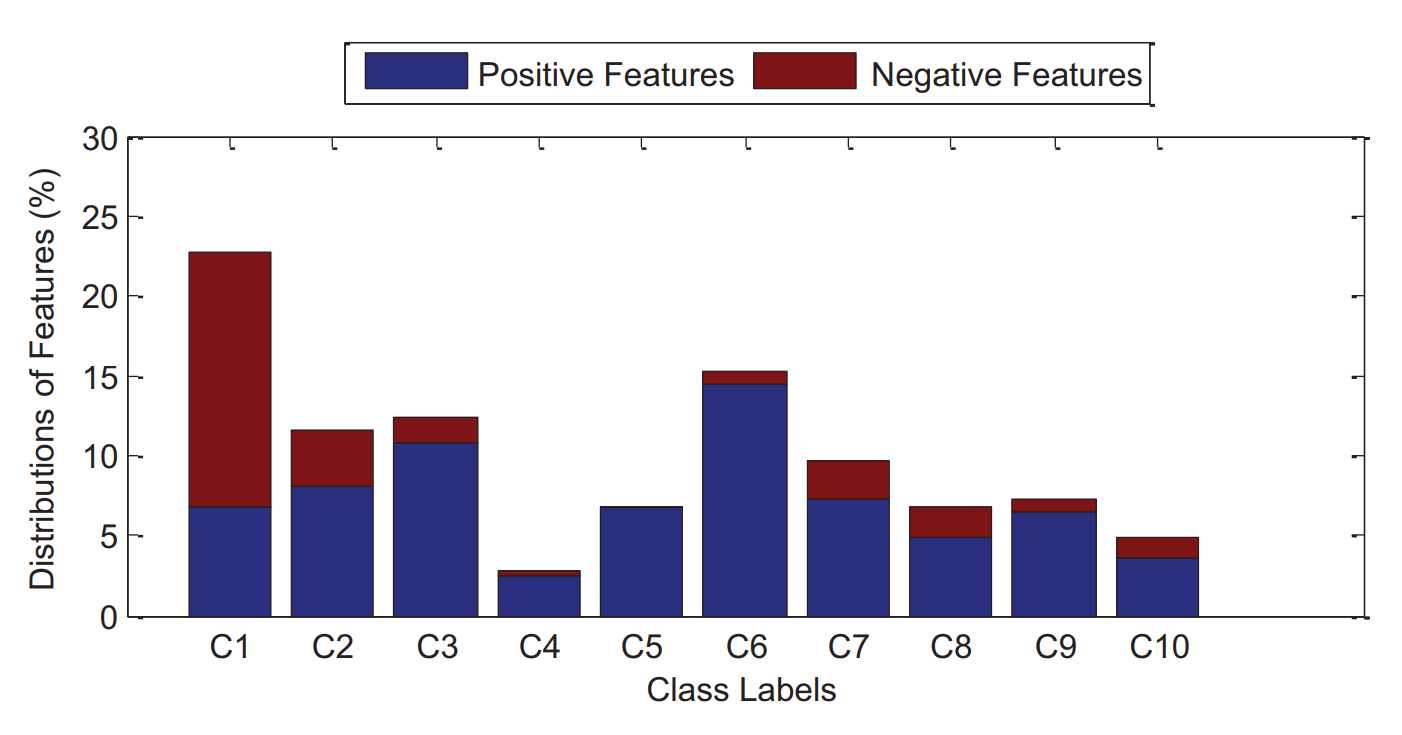
\includegraphics[height=7cm]{IGFSS1.png}
\end{center}
\caption{فراوانی ویژگی‌های انتخاب‌شده نسبت به هر کلاس برای شاخص جینی در روش \lr{IGFSS} \cite{uysal2016improved} }
\end{figure}

در جدول ۴-۱ و ۴-۲ به ترتیب دقت مربوط به روش‌های مختلف انتخاب ویژگی برای دسته‌بند \lr{SVM} و \lr{Naive bayes} بدون استفاده از روش \lr{IGFSS} و با استفاده از آن آورده شده است. با بررسی کلی در می‌یابیم که استفاده از روش پیشنهادی در مقاله منجر به بهبود روش پایه می‌شود اما این بهبود چندان موثر نیست و در هیچ یک از موارد شاهد بیش از ۲ درصد بهبود نیستیم.

\begin{table}
\begin{center}
\caption{معیار $F_1$ برای روش‌های پایه و \lr{IGFSS} برای دسته‌بند \lr{SVM} \cite{uysal2016improved}}
\begin{tabular}{r|r|r|r|r|r|r|r}
\toprule
\textbf{روش} & \textbf{\lr{nfr}} & \textbf{۲۵۰} & \textbf{۳۰۰} & \textbf{۳۵۰} & \textbf{۴۰۰} & \textbf{۴۵۰} & \textbf{۵۰۰}  
\\
\hline
\hline
\lr{IG} & - & ۸۵/۷۵۵ & ۸۶/۰۰۶ & ۸۶/۰۰۶ & ۸۵/۸۶۳ & ۸۶/۰۰۶ & ۸۵/۸۲۷
\\
\lr{IG+IGFSS} & ۰/۶ & ۸۵/۳۶۱ & ۸۶/۴۷۳ & ۸۶/۱۵۰ & ۸۶/۲۹۴ & ۸۶/۱۱۴ & ۸۶/۰۰۶
\\
\lr{GI} & - & ۸۵/۹۳۵ & ۸۵/۹۷۱ & ۸۶/۰۰۶ & ۸۶/۴۰۱ & ۸۶/۰۷۸ & ۸۶/۴۳۷
\\
\lr{GI+IGFSS} & ۰/۳ & 85/648 & 85/791 & 86/329 & 86/437 & 86/760 & 85/935
\\
\lr{DFS} & - & 85/899 & 85/899 & 85/971 & 85/791 & 85/899 & 85/791
\\
\lr{DFS+IGFSS} & ۰/۸ & 85/002 & 86/258 & 86/473 & 86/258 & 86/114 & 85/863
\\
\bottomrule
\end{tabular}
\end{center}
\end{table}

\begin{table}
\begin{center}
\caption{معیار $F_1$ برای روش‌های پایه و \lr{IGFSS} برای دسته‌بند \lr{NB} \cite{uysal2016improved}}
\begin{tabular}{r|r|r|r|r|r|r|r}
\toprule
\textbf{روش} & \textbf{\lr{nfr}} & \textbf{۲۵۰} & \textbf{۳۰۰} & \textbf{۳۵۰} & \textbf{۴۰۰} & \textbf{۴۵۰} & \textbf{۵۰۰}  
\\
\hline
\hline
\lr{IG} & - & 83/531 & 82/382 & 82/382 & 82/562 & 81/916 & 81/737
\\
\lr{IG+IGFSS} & ۰/۶ & 84/105 & 84/284 & 84/320 & 84/212 & 84/535 & 84/033
\\
\lr{GI} & - & 84/535 & 84/212 & 83/961 & 84/141 & 83/674 & 83/423
\\
\lr{GI+IGFSS} & ۰/۳ & 85/109 & 85/468 & 84/822 & 84/966 & 84/356 & 84/571
\\
\lr{DFS} & - & 84/930 & 84/284 & 84/033 & 83/889 & 83/602 & 83/100
\\
\lr{DFS+IGFSS} & ۰/۸ & 84/607 & 85/181 & 85/289 & 84/679 & 84/787 & 84/751
\\
\bottomrule
\end{tabular}
\end{center}
\end{table}

\subsection{دقت روش \lr{MDRC}}
در تصویر ۴-۲ دقت متناسب با معیار $F_1$ برای روش‌های مختلف پایه به همراه روش \lr{MDRC} برای سه روش دسته‌بندی آورده شده است. از این نمودارها می‌توان دریافت که به ازای تعداد ویژگی کم این روش برتری جدی‌ای نسبت به روش‌های پیشین ندارد اما وقتی تعداد ویژگی‌ها بیشتر می‌شود برتری آن نسبت به سایر روش‌ها کاملا حس می‌شود. همچنین می‌توان دید که روش \lr{MDRC} نسبت به سایر روش‌ها برای حالات بیش‌تر از ۵۰۰ ویژگی حداقل ۱۰ درصد بهبود دارد. این بهبود واقعا قابل ملاحظه است و چیزی است که در روش \lr{IGFSS} مشاهده نشده بود؛ لذا می‌توان گفت که به نظر می‌رسد روش \lr{MDRC} دقت بهتری نسبت به روش \lr{IGFSS} دارد.

\begin{figure}[!h]
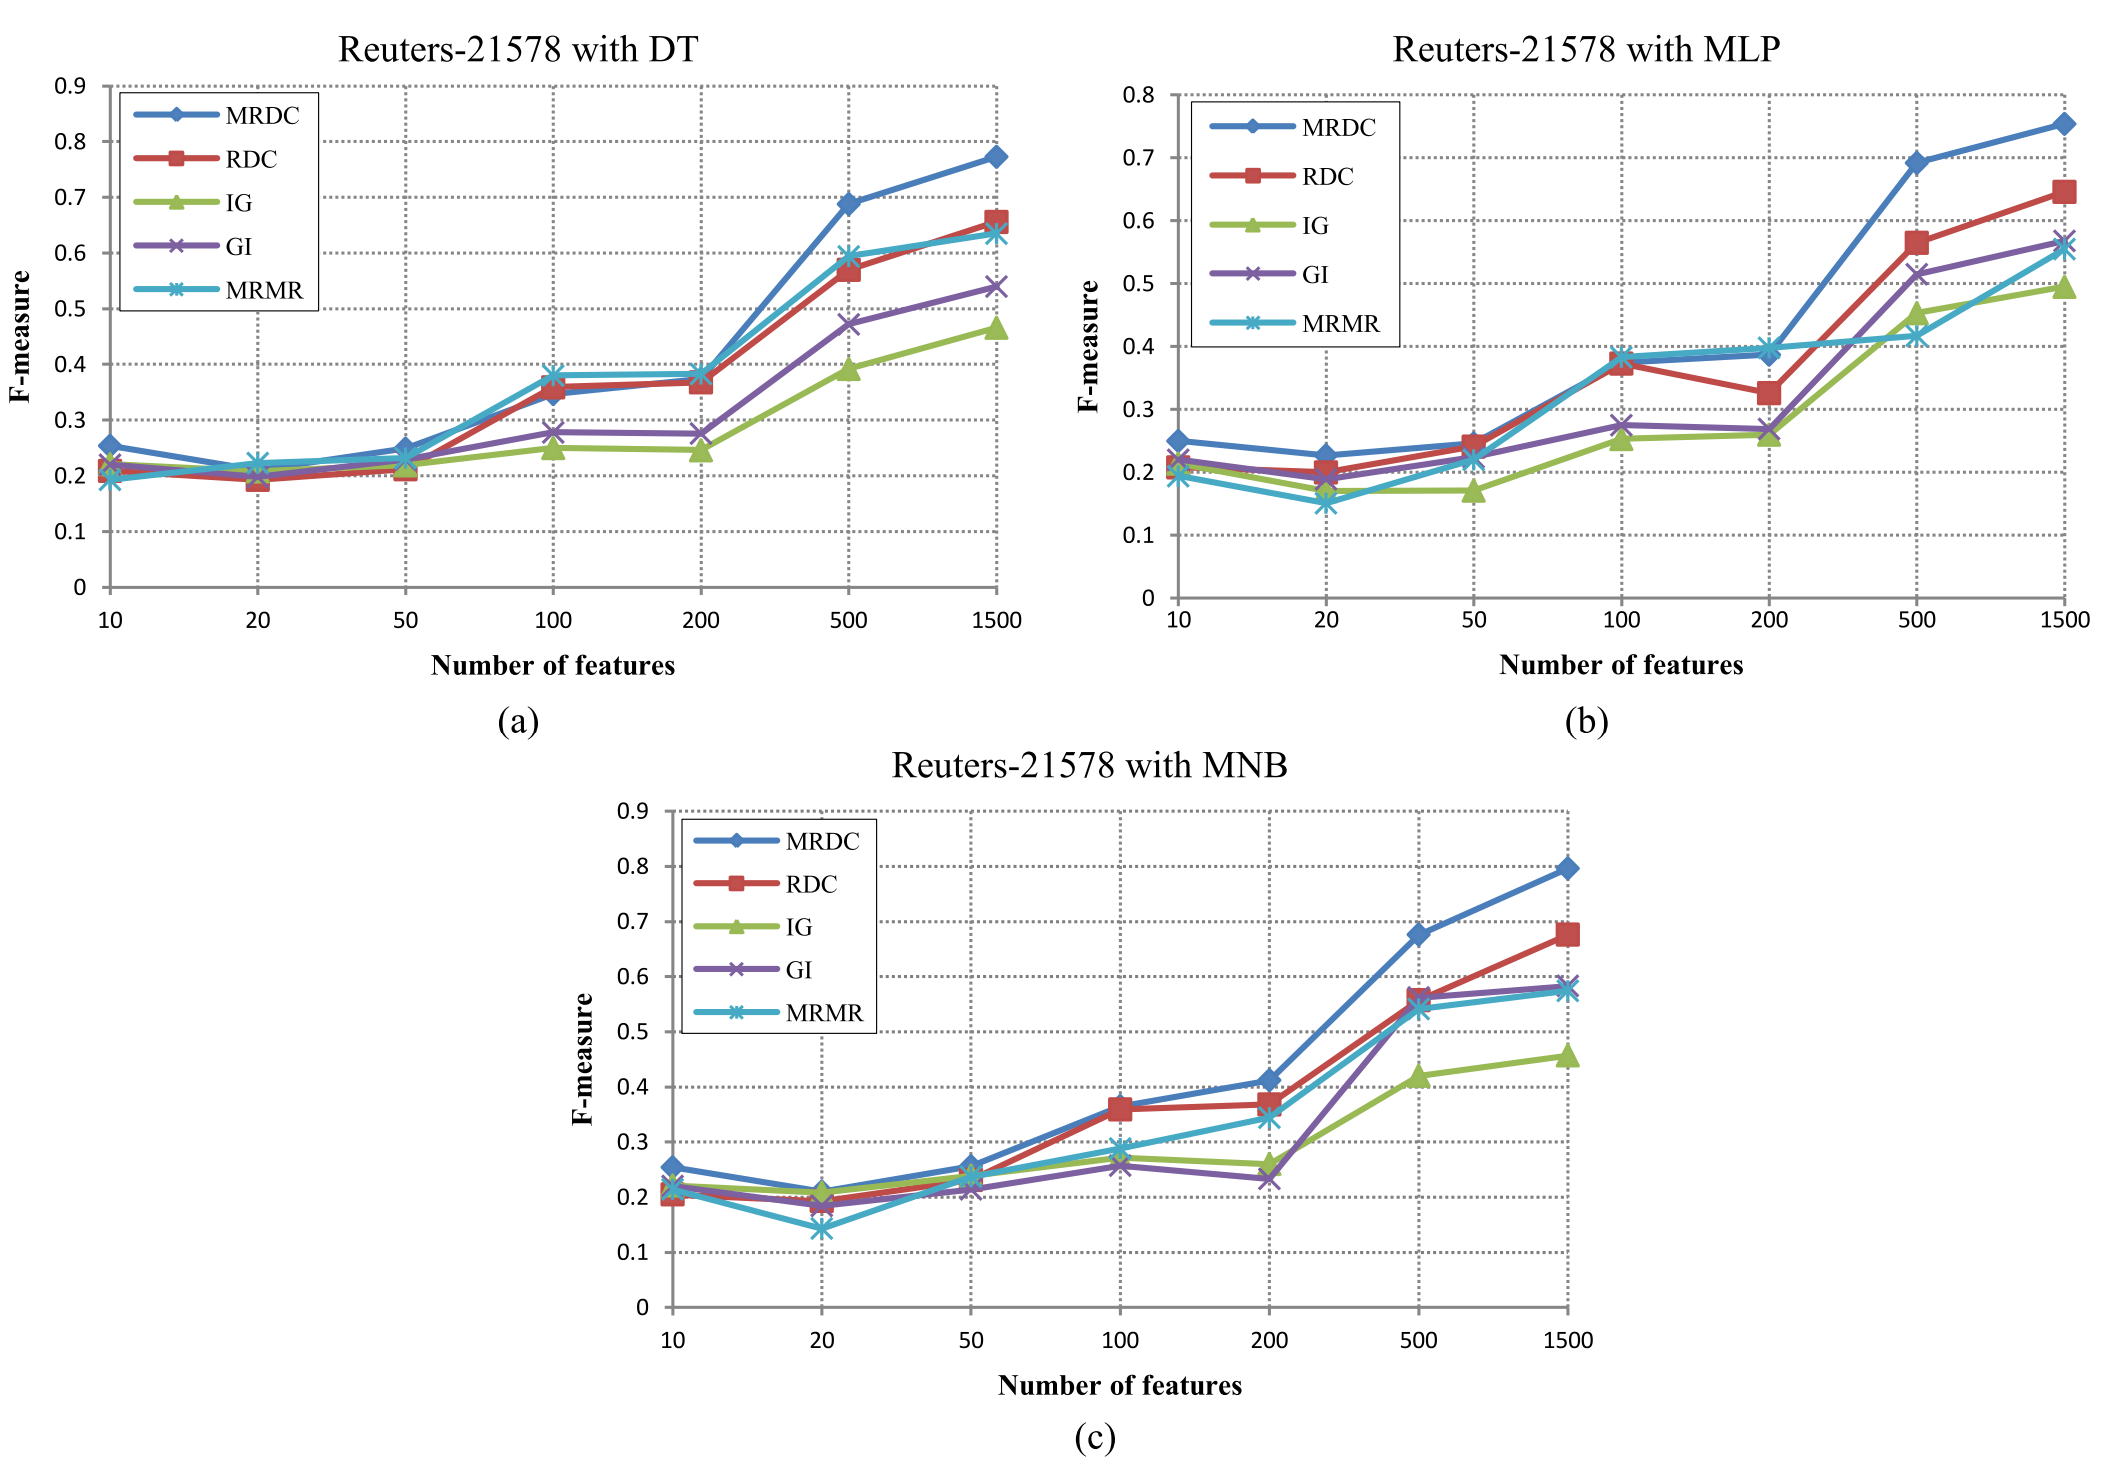
\includegraphics[height=12cm]{MRDC1.png}
\caption{امتیاز معیار $F_1$ برای روش‌های مختلف انتخاب ویژگی و روش \lr{MDRC} و روش‌های دسته‌بندی \lr{(a)} درخت تصمیم \lr{(b)} روش \lr{MLP} \lr{(c)} روش \lr{MNB} \cite{labani2018novel} }
\end{figure}
\chapter{جمع‌بندی و نتیجه‌گیری}
در این پروژه سه روش برای انتخاب ویژگی در مسائل دسته‌بندی متن بررسی شد: روش \lr{IGFSS} آیسال\cite{uysal2016improved}، روش \lr{MRDC} لبنی و همکاران\cite{labani2018novel} و روش بر پایه الگوریتم ژنیتک غارب و همکاران\cite{ghareb2016hybrid}. ایده موجود در روش \lr{IGFSS} حول آن بود که کلاس‌های مختلف سهم برابری در تعداد ویژگی‌ها داشته باشند و همچنین باید به ویژگی‌‌هایی که برای شناخت عدم عضویت به یک کلاس استفاده می‌شود اهمیت داد؛ در اصل باید سهم ویژگی‌های مثبت و منفی از یکدیگر جدا باشد. در روش \lr{MRDC} ایده اصلی آن بود که همبستگی ویژگی‌ها با یکدیگر مورد توجه باشد و به صورت مستقل ویژگی‌ها انتخاب نشوند. نهایتا در روش بر پایه ژنتیک، از الگوریتم ژنتیک برای بهبود خروجی روش‌های انتخاب ویژگی کمک گرفته شد.
\\

با بررسی تئوری و توجه به اعدادی که در مقاله گزارش شده بود، دریافتیم که روش بر پایه ژنتیک خلاقیت بهتری دارد ولی از نظر سرعت و حافظه چندان مناسب نیست. در میان دو روش دیگر، روش \lr{IGFSS} سرعت بهتر و خلاقیت بیشتری داشته است ولی از نظر دقت در جایگاه پایین‌تری بوده است.
\\

در این پروژه تنها سه روش جدید برای بهبود انتخاب ویژگی در مسائل دسته‌بندی مطرح شد. قطعا روش‌های بیشتری را می‌توان مطالعه و بررسی کرد. هیچگاه نمی‌توان یک روش را از تمام لحاظ و برای تمام مجموعه‌های داده و متناسب از روش دیگری برتر دانست. در این شرایط باید روش‌های مختلف را برای کاربرد‌های مختلف مورد ارزیابی قرار داد و نمی‌توان تنها بر یک روش تکیه کرد؛ لذا بررسی بیشتر روش‌ها همچنان سودمند است.
\\

با بررسی همین سه روش، امکان توسعه روش‌های ترکیبی بر مبنای آن‌ها وجود دارد و خود می‌توان یک کار تحقیقاتی مجزا باشد. یعنی آنکه می‌توان ابتدا با دو روش \lr{IGFSS} و روش \lr{MRDC} یک مجموعه ویژگی اولیه ایجاد کرد و سپس با الگوریتم بر پایه ژنتیک این مجموعه را بهبود داد. همچنین می‌توان این سه روش و سایر روش‌ها را به صورت موازی اجرا کرد و برای یک مسئله خروجی را مدنظر قرار داد که دقت بهتری در مسئله دسته‌بندی داشته است. بدین شکل اگرچه حافظه و زمان بیشتری استفاده می‌شود اما دقت نهایی بالاتر خواهد بود. 

%--------------------------------------------------------------------------appendix( مراجع و پیوست ها)
\chapterfont{\vspace*{-2em}\centering\LARGE}%

\appendix
\bibliographystyle{plain-fa}
\bibliography{references}
\chapter*{‌پیوست}
\markboth{پیوست}{}
\addcontentsline{toc}{chapter}{پیوست}
موضوعات مرتبط با متن گزارش پایان نامه كه در يكی از گروه‌های زير قرار می‌گيرد، در بخش پيوست‌ها آورده شوند:
\begin{enumerate}
\item  اثبات های رياضی يا عمليات رياضی طولانی‌.‌
\item داده و اطلاعات نمونه (های) مورد مطالعه (\lr{Case Study}) چنانچه طولانی باشد‌.‌
\item نتايج كارهای ديگران چنانچه نياز به تفصيل باشد‌.‌
\item مجموعه تعاريف متغيرها و پارامترها، چنانچه طولانی بوده و در متن به انجام نرسيده باشد‌.‌
\end{enumerate}
% براي شماره‌گذاري روابط، جداول و اشكال موجود در پيوست‌ از ساختار متفاوتي نسبت به متن اصلي استفاده مي‌شود كه در زير به‌عنوان نمونه نمايش داده شده‌است. 
% \begin{equation}
%F=ma
%\end{equation}
\section*{کد میپل }
\begin{latin}
\begin{verbatim}

with(DifferentialGeometry):
with(Tensor):
DGsetup([x, y, z], M)
																	frame name: M
a := evalDG(D_x)
																	D_x
b := evalDG(-2 y z D_x+2 x D_y/z^3-D_z/z^2)


\end{verbatim}
\end{latin}
%--------------------------------------------------------------------------dictionary(واژه نامه ها)
%اگر مایل به داشتن صفحه واژه‌نامه نیستید، خط زیر را غیر فعال کنید.
\parindent=0pt
%
\chapter*{واژه‌نامه‌ی فارسی به انگلیسی}
\pagestyle{style9}

\addcontentsline{toc}{chapter}{واژه‌نامه‌ی فارسی به انگلیسی}
%%%%%%
\begin{multicols*}{2}

{\bf آ}
\vspace*{3mm}


\farsiTOenglish{اسکالر}{Scalar}


\vspace*{3mm}
{\bf ب}
\vspace*{3mm}

\farsiTOenglish{بالابر}{Lift}


\vspace*{3mm}
{\bf پ}
%%\vspace*{3mm}

\farsiTOenglish{پایا}{Invariant}



\vspace*{3mm}
{\bf ت}
%%\vspace*{3mm}

\farsiTOenglish{ تناظر }{Correspondence}


\vspace*{3mm}
{\bf ث}
%%\vspace*{3mm}

\farsiTOenglish{ثابت‌ساز}{Stabilizer}

\vspace*{3mm}
{\bf ج}
%%\vspace*{3mm}

\farsiTOenglish{جایگشت}{Permutation}



\vspace*{3mm}
{\bf چ}
%%\vspace*{3mm}


\farsiTOenglish{چند جمله‌ای }{Polynomial}

\vspace*{3mm}
{\bf ح}
%%\vspace*{3mm}

\farsiTOenglish{حاصل‌ضرب دکارتی}{Cartesian product}


\vspace*{3mm}
{\bf خ}
%%\vspace*{3mm}

\farsiTOenglish{خودریختی}{Automorphism}

\vspace*{3mm}
{\bf د}
%%\vspace*{3mm}

\farsiTOenglish{درجه}{Degree}


\vspace*{3mm}
{\bf ر}
%%\vspace*{3mm}


\farsiTOenglish{ریزپردازنده}{microprocessor}


\vspace*{3mm}
{\bf ز}
%%\vspace*{3mm}


\farsiTOenglish{زیرمدول}{Submodule}


\vspace*{3mm}
{\bf س}
%%\vspace*{3mm}

\farsiTOenglish{سرشت}{Character}


\vspace*{3mm}
{\bf ص}
%%\vspace*{3mm}

\farsiTOenglish{صادقانه}{Faithful}

\vspace*{3mm}
{\bf ض}
%%\vspace*{3mm}

\farsiTOenglish{ضرب داخلی}{Inner product}

\vspace*{3mm}
{\bf ط}
%%\vspace*{3mm}


\farsiTOenglish{طوقه}{Loop}


\vspace*{3mm}
{\bf ظ}
%%\vspace*{3mm}


\farsiTOenglish{ظرفیت}{Valency}
 
\vspace*{3mm}
{\bf ع}
%%\vspace*{3mm}


\farsiTOenglish{عدم مجاورت}{Nonadjacency}



\vspace*{3mm}
{\bf ف}
%%\vspace*{3mm}

\farsiTOenglish{فضای برداری}{Vector space}



\vspace*{3mm}
{\bf ک}
%%\vspace*{3mm}

\farsiTOenglish{کاملاً تحویل‌پذیر}{Complete reducibility}


\vspace*{3mm}
{\bf گ}
%%\vspace*{3mm}


\farsiTOenglish{گراف}{Graph}



\vspace*{3mm}
{\bf م}
%%\vspace*{3mm}

\farsiTOenglish{ماتریس جایگشتی}{Permutation matrix }


\vspace*{3mm}
{\bf ن}
%%\vspace*{3mm}

\farsiTOenglish{ناهمبند}{Disconnected}


\vspace*{3mm}
{\bf و}
%%\vspace*{3mm}

\farsiTOenglish{وارون‌پذیر}{Invertible}


\vspace*{3mm}
{\bf ه}
%%\vspace*{3mm}

\farsiTOenglish{همبند}{Connected}



\vspace*{3mm}
{\bf ی}
%%\vspace*{3mm}

\farsiTOenglish{یال}{Edge}




\end{multicols*}%
%%%%%%
\chapter*{ واژه‌نامه‌ی انگلیسی به فارسی}
\pagestyle{style9}
\lhead{\thepage}\rhead{واژه‌نامه‌ی انگلیسی به فارسی}
\addcontentsline{toc}{chapter}{واژه‌نامه‌ی انگلیسی به فارسی}

\LTRmulticolcolumns
\begin{multicols}{2}
{\hfill\bf  \lr{A}}
%%\vspace*{1.5mm}

\englishTOfarsi{Automorphism}{خودریختی}

\vspace*{3mm}
{\hfill\bf   \lr{B}}
%%\vspace*{1.5mm}

\englishTOfarsi{Bijection}{دوسویی}

\vspace*{3mm}
{\hfill\bf   \lr{C}}
%%\vspace*{1.5mm}

\englishTOfarsi{Cycle group}{گروه دوری}

\vspace*{3mm}
{\hfill\bf   \lr{D}}
%%\vspace*{1.5mm}

\englishTOfarsi{Degree}{درجه}

\vspace*{3mm}
{\hfill\bf   \lr{E}}
%%\vspace*{1.5mm}

\englishTOfarsi{Edge}{یال}

\vspace*{3mm}
{\hfill\bf   \lr{F}}
%%\vspace*{1.5mm}

\englishTOfarsi{Function}{تابع}

\vspace*{3mm}
{\hfill\bf   \lr{G}}
%%\vspace*{1.5mm}

\englishTOfarsi{Group}{گروه}

\vspace*{3mm}
{\hfill\bf   \lr{H}}
%%\vspace*{1.5mm}

\englishTOfarsi{Homomorphism}{همریختی}

\vspace*{3mm}
{\hfill\bf   \lr{I}}
%%\vspace*{1.5mm}

\englishTOfarsi{Invariant}{پایا}

\vspace*{3mm}
{\hfill\bf   \lr{L}}
%%\vspace*{1.5mm}

\englishTOfarsi{Lift}{بالابر}

\vspace*{3mm}
{\hfill\bf   \lr{M}}
%%\vspace*{1.5mm}

\englishTOfarsi{Module}{مدول}

\vspace*{3mm}
{\hfill\bf   \lr{N}}
%%\vspace*{1.5mm}

\englishTOfarsi{Natural map}{نگاشت طبیعی}

\vspace*{3mm}
{\hfill\bf   \lr{O}}
%%\vspace*{1.5mm}

\englishTOfarsi{One to One}{یک به یک}

\vspace*{3mm}
{\hfill\bf   \lr{P}}
%%\vspace*{1.5mm}

\englishTOfarsi{Permutation group}{گروه جایگشتی}

\vspace*{3mm}
{\hfill\bf   \lr{Q}}
%%\vspace*{1.5mm}

\englishTOfarsi{Quotient graph}{گراف خارج‌قسمتی}

 \vspace*{3mm}
{\hfill\bf   \lr{R}}
%%\vspace*{1.5mm}

\englishTOfarsi{Reducible}{تحویل پذیر}

\vspace*{3mm}
{\hfill\bf   \lr{S}}
%%\vspace*{1.5mm}

\englishTOfarsi{Sequence}{دنباله}

 \vspace*{3mm}
{\hfill\bf   \lr{T}}
%%\vspace*{1.5mm}

\englishTOfarsi{Trivial character}{سرشت بدیهی}

\vspace*{3mm}
{\hfill\bf   \lr{U}}
%%\vspace*{1.5mm}

\englishTOfarsi{Unique}{منحصربفرد}

\vspace*{3mm}
{\hfill\bf   \lr{V}}
%%\vspace*{1.5mm}

\englishTOfarsi{Vector space}{فضای برداری}
\end{multicols}
%--------------------------------------------------------------------------index(نمایه)
%اگر مایل به داشتن صفحه نمایه نیستید، خط زیر را غیر فعال کنید.
\pagestyle{style7}
\printindex
\pagestyle{style7}
%کلمات کلیدی انگلیسی
\latinkeywords{Write a 3 to 5 KeyWords is essential. Example: AUT, M.Sc., Ph. D,..}
%چکیده انگلیسی

\en-abstract{
This page is accurate translation from Persian abstract into English.
}
%%%%%%%%%%%%%%%%%%%%% کدهای زیر را تغییر ندهید.

\newpage
\thispagestyle{empty}
\begin{latin}
\section*{\LARGE\centering Abstract}

\een-abstract

\vspace*{.5cm}
{\large\textbf{Key Words:}}\par
\vspace*{.5cm}
\elatinkeywords
\end{latin}
% در این فایل، عنوان پایان‌نامه، مشخصات خود و چکیده پایان‌نامه را به انگلیسی، وارد کنید.
%%%%%%%%%%%%%%%%%%%%%%%%%%%%%%%%%%%%
\baselineskip=.6cm
\begin{latin}

\latinfaculty{Department of ...}


\latintitle{Title of Thesis}


\firstlatinsupervisor{Dr. }

%\secondlatinsupervisor{Second Supervisor}

\firstlatinadvisor{Dr. }

%\secondlatinadvisor{Second Advisor}

\latinname{Name}

\latinsurname{Surname}

\latinthesisdate{Month \& Year}

\latinvtitle
\end{latin}

\end{document}